\subsection*{Поглощение веществ}

\paragraph*{}В процессе жизнедеятельности, растение поглощает из окружающей среды вещества, включающие в себя различные химические элементы. При этом, надо понимать, что значительная часть этих химических элементов необходимы растению для нормальной жизнедеятельности и не могут быть заменены на какие либо \hyperlink{libihBarell}{другие}. Такие, незаменимые химические элементы называются \gls{nutrientElements}. А соединения, в состав которых входят питательные элементы носят название \gls{nutrients}. Для растения питательными веществами служат минеральные соли, содержащиеся в почве.

\paragraph*{}\gls{nutrientElements} могут содержаться в почве в следующих формах: 

\begin{enumerate}

\item В недоступной для растения форме

	\begin{enumerate}

		\item В виде прочно фиксированных в различных минералах веществ; \note{например, ионы $K^{+}$ и $NH^{+}_{4}$ в некоторых глинистых минералах \cite{malinowsky_2004}}
		\item В виде труднорастворимых неорганических солей; \note{например различные сульфаты, фосфаты, карбонаты}

	\end{enumerate}
	
\item В доступной для растения форме

	\begin{enumerate}

		\item В виде адсорбированных на поверхности коллоидов, доступных для растений благодаря \hyperlink{contact_exchanging}{ионному обмену};
		\item В виде растворенных в воде и поэтому легко доступных для растений;

	\end{enumerate}

\end{enumerate}

\paragraph*{}Поглощаемые растением ионы поступают в клетки \hyperlink{question_rizoderma}{ризодермы} следующими путями:

\begin{enumerate}
	\item Непосредственно из почвенного раствора
	\item Благодаря контактному обмену $H^{+}$, $HCO^{-}_{3}$ и анионов органических кислот на ионы минеральных веществ почвенных частиц.
\end{enumerate} 

\subsubsection*{Поглощение веществ путем контактного обмена}

\paragraph*{}\note{Обменные катионы и анионы -- один из важнейших источников питания для растений}

\paragraph*{}При \hypertarget{contact_exchanging}{контактном обмене}, растение обменивает катионы и анионы, находящиеся на частицах почвы на ионы, адсорбированные на поверхности клеток корня. 

\paragraph*{}Путем контактного обмена может происходить поступление как катионов, так и анионов. Так, при поглощении катионов  $K^{+}$, $Ca^{2+}$, $Na^{+}$ растение обменивает их на \gls{proton}ы $H^{+}$. Анионы $NO^{-}_{3}$, $PO^{3-}_{4}$ поступают в корень в обмен на гидрокарбонат-ионы $HCO^{-}_{3}$ или анионы органических кислот. 

\paragraph*{}Контактный обмен ионов между \hyperlink{cell_wall}{клеточными стенками} клеток ризодермы и частицами почвы осуществляется без перехода ионов в почвенный раствор. Необходимый для этого тесный контакт между частицами почвы и клетками ризодермы обеспечивается благодаря следующим механизмам:

\begin{enumerate}
	\item Выделению слизи корневыми волосками
	\item Отсутствию у ризодермы кутикулы и других защитных покровов
\end{enumerate}
 
%Так как адсорбированные ионы находятся в постоянном колебательном движении и занимают определенный объем - сферу колебаний, при тесном контакте поверхностей сферы колебаний двух ближайших адсорбированных ионов могут перекрываться, в результате чего осуществляется ионный обмен. 
%Выделяя различные вещества (углекислый газ, аминокислоты, сахара и другие), корень растения изменяет состояние питательных веществ в прикорневой зоне непосредственно, например, путем выделения СО2 (СО2 + Н2О Н+ + НСО-3: повышение растворимости фосфатов и карбонатов) и косвенно, создавая благоприятные условия для ризосферы, которая играет большую роль в превращении почвенных минералов.

\paragraph*{}В целом, можно отметить следующие особенности поглощения растением минеральных веществ: 

\begin{enumerate}
	\item Количество минеральных веществ, поступивших в растение и накапливающихся в нем, не \hyperlink{what_is_transport_type}{пропорционально} количеству прошедшей через растение воды.
	\item Из очень разбавленных растворов соли поглощаются быстрее, чем вода.
	\item Из концентрированных растворов в растение быстрее поступает вода.
	\item Минеральные соли и вода поступают в растение относительно независимо друг от друга и с помощью различных механизмов.
\end{enumerate}

\subsubsection*{Этапы поглощения веществ}

\paragraph*{}Путь иона из почвенного раствора в органеллы клетки можно представить как последовательность следующих событий:

\begin{enumerate}

	\item Поступление ионов из почвенного раствора или из свободного пространства соседней клетки в свободное пространство \hyperlink{cell_wall}{клеточной стенки} ризодермы;
	\item Транспорт ионов через \hyperlink{plasmolema}{цитоплазмотическую мембрану} клетки в цитоплазму.
	\item Транспорт ионов в различные органеллы клетки через их мембраны. 

\end{enumerate}

\paragraph*{}Непосредственно через саму \hyperlink{plasmolema}{цитоплазматическую мембрану} ионы и \hyperlink{polarMolecula}{полярные молекулы} проникнуть не могут. Это связанно с тем, что:

\begin{enumerate}

	\item Внутренняя часть двойного липидного слоя мембраны гидрофобна и через нее заряженные частицы проникнуть не способны;
	\item Внешняя сторона цитоплазматической мембраны, в свою очередь, имеет электрический заряд. Так, поверхность \hyperlink{plasmolema}{плазмалеммы} заряжена отрицательно а поверхность \hyperlink{cell_vakuol}{тонопласта} -- положительно. По этой причине поверхность мембраны будет отталкивать одноименно заряженные ионы;
	\item Находящиеся в растворе ионы окружены гидратными оболочками, увеличивающими их размер.
	\item Концентрация веществ в клетке больше, чем в свободном пространстве, т.е. вещество должно двигаться против градиента концентрации.  

\end{enumerate}

\paragraph*{}Для того, чтобы растворенные в воде вещества смогли пройти через мембрану клетки в ней есть поры, образованные специальными \hyperlink{proteins}{белками}. 

\subsubsection*{Механизмы транспорта}

\paragraph*{}Различные механизмы транспорта веществ через мембрану можно разделить на следующие типы:

\begin{enumerate}

\item \gls{passiveTranspotr} -- это транспорт через мембрану без затраты энергии (в виде молекул \gls{atp}). При пассивном транспорте движение ионов происходит по градиенту электрохимического потенциала (\ris \ref{celltransport}). Основным механизмом пассивного транспорта является \gls{diffusion}.
	
\item \gls{activeTranspotr} -- это транспорт, идущий против электрохимического потенциала с затратой энергии (в виде молекул \gls{atp}), выделяющейся в процессе \gls{metabolism}а (\ris \ref{celltransport}). Основными механизмами активного транспорта являются:
	
	\begin{enumerate}
	
		\item Везикулярный транспорт, включающий \Gls{endocytosis}, экзоцитоз
		\item Молекулярный транспорт, происходящий через мембранные транспортные белки (белки-переносчики и каналообразующие белки).
	
	\end{enumerate}

\end{enumerate}

%%%%%%%%%%%%%%%%%%%%%%%%%%%%%%%%%%%%%%%%%%%%%%%%%%%%%%%%%%%%%%%%%%%%%%%%%%%%%%%%%%%%%%%%%%%%%%%%%%%%%%%%%%% 
\begin{figure}[h!]
  \centering
       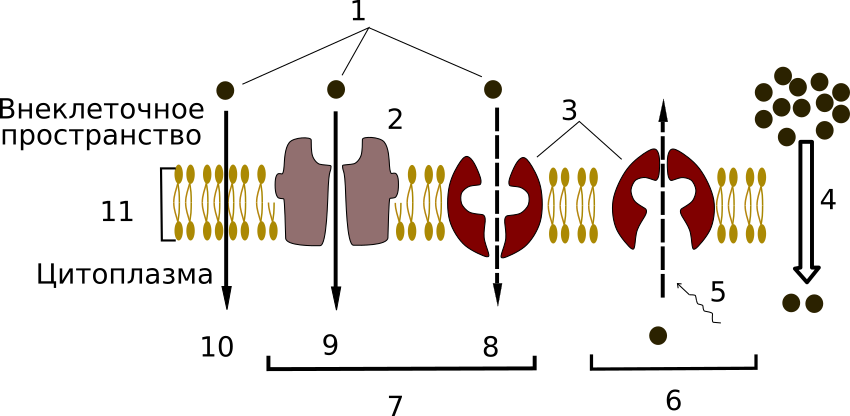
\includegraphics[width=0.7\linewidth]{pictures/celltransport}
\caption{Активный и пассивный транспорт вещество через цитоплазматическуцю мембрану}


\paragraph*{}1. Транспортируемая молекула; 2. Каналобразующий белок; 3. Белок переносчик; 4. Электрохимический градиент; 5. Энергия; 6. \gls{activeTranspotr}; 7. \gls{passiveTranspotr}; 8. \gls{diffusion} с помощью белка-переносчика; 9. \gls{diffusion} через канал; 10. Простая диффузия 11. Липидный слой. 

\paragraph*{}Рисунок приведен согласно Альбертсу Б \cite{alberts_2013}

\label{celltransport}
\end{figure}
%%%%%%%%%%%%%%%%%%%%%%%%%%%%%%%%%%%%%%%%%%%%%%%%%%%%%%%%%%%%%%%%%%%%%%%%%%%%%%%%%%%%%%%%%% 

\paragraph*{Пассивный транспорт}

\paragraph*{}Один из важнейших видов пассивного транспорта через мембраны -- это диффузия. \hypertarget{diffusion}{\gls{diffusion}} -- это самопроизвольное проникновение одного вещества в другое при их соприкосновении. Движение вещества путем диффузии происходит по градиенту концентрации; 

\paragraph*{}Путем диффузии в свободное пространство клеточной стенки поступают:

\begin{enumerate}
	\item вещества, растворимые в жирах
	\item $O_{2}$, $CO_{2}$
	\item этанол
\end{enumerate}

\paragraph*{}Через цитоплазматическую мембрану эти вещества попадают через специальные белки-\gls{porins}
 
%Закон диффузии: молекулы газа или растворенного вещества двигаются туда, где их меньше, т.е. по градиенту концентрации.

\paragraph*{}Белки-\gls{porins} (\ris \ref{porin}) -- образуют в липидном бислое мембраны <<поры>>, заполненные водой. Внутренняя поверхность этих белков гидрофильна, что позволяет проходить через нее молекулам воды и ионам. Внешняя же часть белка гидрофобна, что позволяет ему закрепится в липидном слое мембраны. Поры, образованные белками, могут открываться на короткое время и закрываться. Белковые каналы плазмалеммы обладают избирательностью, т.е. через них могут проходить ионы только определенного вида и размера.

%%%%%%%%%%%%%%%%%%%%%%%%%%%%%%%%%%%%%%%%%%%%%%%%%%%%%%%%%%%%%%%%%%%%%%%%%%%%%%%%%%%%%%%%%%%%%%%%%%%%%%%%%%% 
\begin{figure}[h!]
  \centering
       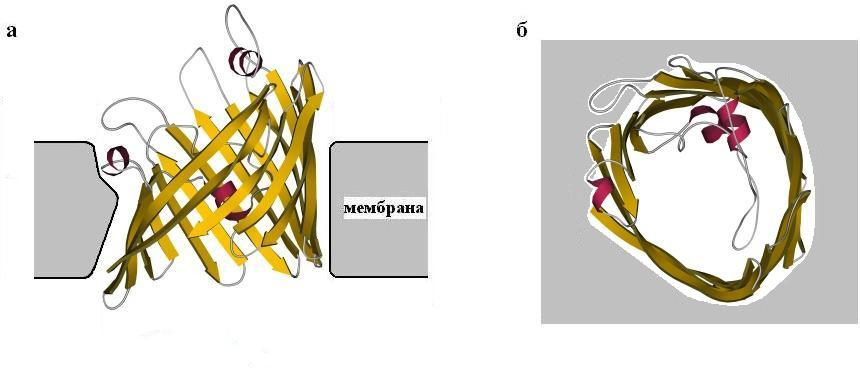
\includegraphics[width=0.5\linewidth]{pictures/porin}
\caption{Структура белка-порина}
\label{porin}
\end{figure}
%%%%%%%%%%%%%%%%%%%%%%%%%%%%%%%%%%%%%%%%%%%%%%%%%%%%%%%%%%%%%%%%%%%%%%%%%%%%%%%%%%%%%%%%%% 

\note{Через каналы, образованные белками, ионы транспортируются со скоростью 106 ионов в сек, т.е. в 1000 раз быстрее, чем с помощью белка-переносчика. Транспорт через каналы является всегда пассивным \cite{malinowsky_2004}}

\paragraph*{Активный транспорт}

\paragraph*{}Мембранные транспортные белки переносят маленькие водорастворимые молекулы (сахара, аминокислоты, нуклеотиды и др.)

\paragraph*{}\remember{Белки-переносчики переносят растворенные вещества через цитоплазматическую мембрану, изменяя свою форму, при этом участки белка, с которыми связывается ион, открываются то с одной, то с другой стороны мембраны}

\paragraph*{}У высших растений большое значение имеет деятельность такого белка переносчика, как протонная помпа. \gls{protonsPomp} -- это интегральный мембранный белок, осуществляющий перемещение \gls{proton}ов через мембрану.  Поскольку насос прокачивает протоны против градиента их концентрации, процесс идет с затратой \gls{atp} или \gls{nadfh2}. Вынос протонов на внешнюю сторону цитоплазматической мембраны сопровождается поступлением внутрь клетки катионов. Вместе с \gls{proton}ами в ту же сторону могут передвигаться и анионы.

\paragraph*{}\Gls{endocytosis} -- это активный способ поглощение макромолекул клеткой, сопровождающийся впячиванием участков мембраны и образованием везикул.  В ходе эндоцитоза происходит следующая последовательность событий (\ris \ref{endocytoze}):

\begin{enumerate}

	\item Поглощаемые клеткой макромолекулы адсорбируются на поверхности клеточной мембраны (\ris \ref{endocytoze} I);  
	\item Небольшой участок мембраны впячивается, окружая транспортируемое вещество (\ris \ref{endocytoze} II);
	\item В результате смыкания краев впячивания мембраны, образуя внутриклеточный пузырек -- \gls{vesicula} III;
	\item \gls{vesicula} отделяется от мембраны (например, плазмалеммы) и передвигается в цитозоле (\ris \ref{endocytoze} IV); 
	\item \gls{vesicula} соединяется с лизосомой, \hyperlink{enzimes}{ферменты} которой или разрушают мембрану везикулы или разрушают само вещество находящиеся внутри везикулы (\ris \ref{endocytoze} V); 
	\item Образовавшиеся мелкие фрагменты содержимого везикулы проходят через мембрану везикулы в цитозоль

\end{enumerate}

%%%%%%%%%%%%%%%%%%%%%%%%%%%%%%%%%%%%%%%%%%%%%%%%%%%%%%%%%%%%%%%%%%%%%%%%%%%%%%%%%%%%%%%%%%%%%%%%%%%%%%%%%%% 
\begin{figure}[h!]
  \centering
       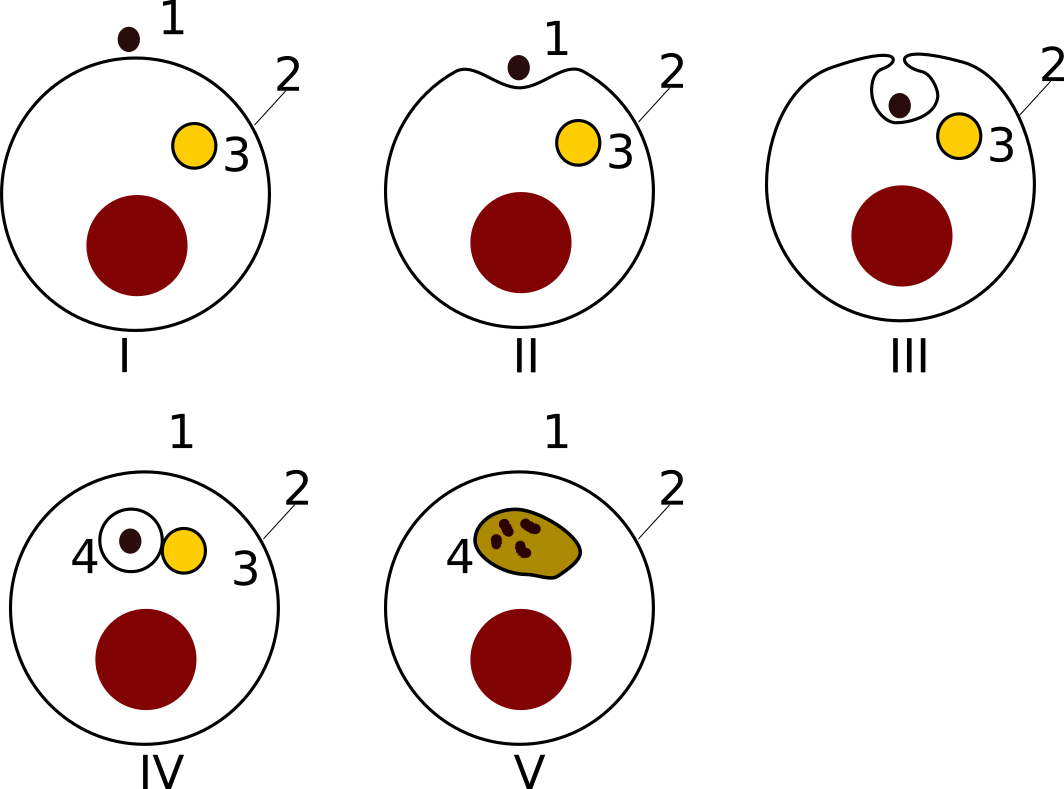
\includegraphics[width=0.7\linewidth]{pictures/endocytoze}
\caption{Стадии эндоцитоза}
\label{endocytoze}
\end{figure}
%%%%%%%%%%%%%%%%%%%%%%%%%%%%%%%%%%%%%%%%%%%%%%%%%%%%%%%%%%%%%%%%%%%%%%%%%%%%%%%%%%%%%%%%%% 

\subsection*{Влияние факторов окружающей среды на активность поглощения минеральных веществ}

\subsubsection*{Температура}

\paragraph*{}При температуре, близкой к 0 \celsius, поглощение солей идет медленно, затем, в пределах до 40 \celsius, оно усиливается. Увеличение интенсивности поглощения солей идет согласно правилу Ван-Гоффа -- увеличение температуры на 10 \celsius может вызвать возрастание поглощения в 2-3 раза.

\subsubsection*{Свет}

\paragraph*{}Свет может оказывать на интенсивность поглощения солей как прямое, так и косвенное влияние.

\begin{enumerate}
	\item Прямое влияние заключается в том, что в темноте поглощение солей замедляется и постепенно прекращается, а на свету -- ускоряется. \note{При этом, на прямое влияние света указывает быстрота с которой изменяется скорость поглощения ионов растением}
	\item Косвенное влияние заключается в том, что на свету, в процессе \hyperlink{photosyntesis}{фотосинтеза}, образуются \hyperlink{sect_glycosids}{углеводы}, которые необходимы для \hyperlink{sect_breazing}{дыхания} и образования \gls{atp}, энергия которой используется на поступление веществ. 
\end{enumerate}

\subsubsection*{Концентрация кислорода}

\paragraph*{}При уменьшении содержания кислорода до 2—3\% интенсивность поступления солей остается на одном уровне. Лишь снижение концентрации кислорода ниже 3\% вызывает падение поглощения примерно в два раза. 

%\paragraph*{}Поглощение одного иона зависит от присутствия других ионов. Так, в присутствии легко поглощаемого аниона катионы той же соли поступают быстрее. Ионы с одинаковым зарядом обычно конкурируют между собой.

\subsubsection*{Влияние внутренних факторов на поступление солей} 

\paragraph*{}На интенсивность поступления минеральных веществ в корень оказывают влияние такие внутренние факторы, как:

\begin{enumerate}
	\item Интенсивность \hyperlink{sect_breazing}{дыхания}. При этом можно выделить следующие направления влияния
	\begin{enumerate}
		\item В процессе \hyperlink{sect_breazing}{дыхания} выделяется углекислый газ, который в воде образует угольную кислоту. Адсорбируясь на поверхности корня, эти ионы служат обменным фондом для поступающих катионов и анионов.
%		\item В процессе переноса ионов через мембрану участвуют специфические ё	ся в зависимости от интенсивности дыхательного процесса.
		\item В процессе дыхания накапливается энергия (в форме макроэргических связей \gls{atp}), необходимая для активного поступления ионов
	\end{enumerate}	
	\item Наличие токсинов-ингибиторов дыхания. Ингибиторы процесса \hyperlink{sect_breazing}{дыхания} (в частности, цианистый калий) резко тормозят поступление солей. 
	
\end{enumerate}

\note{Сопоставление количества воды, испаренной в процессе транспирации, и количества поступивших солей показывает, что прямой зависимости между этими процессами обычно нет \cite{malinowsky_2004}} 



%4.2. Содержание минеральных элементов в растениях

%Растения способны поглощать из окружающей среды практически все элементы. Однако для нормальной жизнедеятельности растительному организму необходимо лишь 19 питательных элементов. Среди них углерод (45 \% сухой массы тканей), кислород (42\%), водород (6,5\%) и азот (1,5\%) называют органогенами. Оставшиеся 5 \% приходятся на зольные элементы, которые остаются в золе после сжигания растения. Содержание минеральных элементов обычно выражают в процентах от массы сухого вещества. Все элементы в зависимости от их количественного содержания в растении принято делить на макроэлементы (содержание более 0,01 \%) - к ним относятся азот, фосфор, сера, калий, кальций, магний и микроэлементы (содержание менее 0,01 \%): железо, марганец, медь, цинк, бор, молибден, кобальт, хлор. Ю. Либихом было установлено, что все перечисленные элементы равнозначны и полное исключение любого из них приводит растение к глубокому страданию и гибели, ни один из перечисленных элементов не может быть заменен другим, даже близким по химическим свойствам. Макроэлементы при концентрации 200-300 мг/л в питательном растворе еще не оказывают вредного действия на растение. Большинство микроэлементов при концентрации 0,1-0,5 мг/л угнетают рост растений.
%Для нормальной жизнедеятельности растений должно быть определенное соотношение различных ионов в окружающей среде. Чистые растворы одного какого-либо катиона оказываются ядовитыми. Так, при помещении проростков пшеницы на чистые растворы KCL или CaCL2 на корнях сначала появлялись вздутия, а затем корни отмирали. Смешанные растворы этих солей не обладали ядовитым действием. Смягчающее влияние одного катиона на действие другого катиона называют антагонизмом ионов. Антагонизм ионов проявляется как между разными ионами одной валентности, например, между ионами натрия и калия, так и между ионами разной валентности, например, калия и кальция. Одной из причин антагонизма ионов является их влияние на гидратацию белков цитоплазмы. Двухвалентные катионы (кальций, магний) дегидратируют коллоиды сильнее, чем одновалентные (натрий, калий). Следующей причиной антагонизма ионов является их конкуренция за активные центры ферментов. Так, активность некоторых ферментов дыхания ингибируется ионами натрия, но их действие снимается добавлением ионов калия. Кроме того, ионы могут конкурировать за связывание с переносчиками в процессе поглощения. Действие одного иона может и усиливать влияние другого иона. Это явление называется синергизмом. Так, под влиянием фосфора повышается положительное действие молибдена. 

\subsection*{Физиологическая роль основных элементов питания}

\subsubsection*{Углерод}

\paragraph*{Физиологическая роль}

\paragraph*{}Является основным компонентом органического вещества, синтезируемого в процессе \hyperlink{photosyntesis}{фотосинтеза}. В процессе \hyperlink{sect_breazing}{дыхания} органические вещества расщепляются. При этом растения потребляют кислород и выделяют углекислый газ. Таким образом, растения участвуют в круговороте углерода на нашей планете. 

\paragraph*{Источники углерода}

\paragraph*{}Растение получает углерод из воздуха, поглощая углекислый газ, 2-5 \% углерода усваивается корнями в виде углекислоты из почвы. 


\subsubsection*{Фосфор}

\paragraph*{Физиологическая роль фосфора}

\paragraph*{}\hypertarget{phosphoros}{Фосфор} входит в состав ряда важнейших органических соединений, таких, как:

\begin{enumerate}

	\item Нуклеиновых кислот;
	\item Нуклеотидов;
	\item \hyperlink{plipids}{Фосфолипидов};
	\item \hyperlink{vitamines}{Витаминов};
	\item \gls{atp}

\end{enumerate}

\paragraph*{}Многие фосфорсодержащие витамины и их производные являются \gls{coenzim}ами.

\paragraph*{}Для фосфора характерна способность к образованию химических макроэргических связей с высоким энергетическим потенциалом. 

%Фосфор входит в состав АТФ, которая является энергетической валютой в живых организмах. 
\paragraph*{}\gls{phosphriling}, то есть присоединении остатка фосфорной кислоты, активирует клеточные белки и углеводы и необходимо для таких процессов, как \hyperlink{sect_breazing}{дыхание}, синтез \gls{rna} и белка, деление и дифференцировка клеток, защитные реакции против патогенов и т.д.

\paragraph*{Источники фосфора}

\paragraph*{}Растения поглощают фосфор из почвы в виде:

\begin{enumerate}

\item Свободной ортофосфорной кислоты 
\item Двух- и однозамещенных солей фосфорной кислоты, 
\item Некоторых органических соединений фосфора, такие как фосфаты сахаров и фитин.

\end{enumerate}
  
%Содержание фосфора в растениях составляет около 0,2 \% на сухую массу. 
%Основной запасной формой фосфора у растений является фитин - кальций-магниевая соль инозитфосфорной кислоты. Содержание фитина в семенах достигает 2 \% от сухой массы, что составляет 50\% от общего содержания фосфора.

\paragraph*{Симптомы недостатка фосфора}

\paragraph*{}При дефиците фосфора: 

\begin{enumerate}

	\item Снижается скорость поглощения кислорода;
	\item Снижается активность дыхательных \hyperlink{enzimes}{ферментов}, локализованных в митохондриях;
	\item Активируются \hyperlink{enzimes}{ферменты} немитохондриальных систем окисления; 
	\item Происходит распад фосфорорганических соединений;
	\item Тормозится синтез белков и свободных нуклеотидов. Наиболее чувствительны к недостатку фосфора молодые растения. 
	\remember{Замедление интенсивности вышеназванных процессов метаболизма при недостатке фосфора связано с уменьшением количества \gls{atp}, которая служит переносчиком энергии, необходимой для осуществления многих реакций и для синтеза которой необходим фосфор}
	\item При недостатке фосфора, листья, особенно старые, приобретают синевато-зеленую окраску, нередко с пурпурным из-за накопления антоцианов или бронзовым оттенком (свидетельство задержки синтеза \hyperlink{proteins}{белка} и накопления сахаров). 
	\item Листья становятся мелкими и более узкими. Приостанавливается рост растений, задерживается созревание урожая;

\end{enumerate}

\subsubsection*{Сера}

\paragraph*{Физиологическая роль серы}

\begin{enumerate}

\item Сера участвует в образовании в образовании ковалентных, водородных и меркаптидных связей, поддерживающих трехмерную структуру белка. \note{Дисульфидные мостики между полипептидными цепями и двумя участками одной цепи (по типу S-S-мостика в молекуле цистеина) стабилизируют молекулу \hyperlink{proteins}{белка}} 

\item Сера входит в состав важнейших аминокислот -- цистеина и метионина (\ris \ref{saminoacids}), которые могут находиться в растениях в свободной форме или в составе белков. \note{Метионин относится к числу 10 незаменимых аминокислот, входит в состав активных центров многих ферментов. Метиониновые остатки могут придавать молекуле \hyperlink{proteins}{белка} гидрофобные свойства, что играет важную роль в стабилизации активной конформации \hyperlink{enzimes}{ферментов} в солевом окружении} 
\item Сера входит в состав многих витаминов и \gls{coenzim}ов, таких как биотин, коэнзим А, глутатион, липоевая кислота. \note{По этой причине сера необходима для многих процессов обмена веществ (например, аэробная фаза дыхания, синтез жиров и так далее)} 
\item Сера участвует в образовании полиаминов, которые влияют на структуру нуклеиновых кислот и рибосом, регулируют процессы деления клеток. 

\end{enumerate}

\paragraph*{Источники серы}

\paragraph*{}Основные неорганические соединения серы в почве -- сульфаты ($CaSO_{4}$, $MgSO_{4}$, $Na_{2}SO_{4}$). В затопляемых почвах сера находится в восстановленной форме в виде $FeS$, $FeS_{2}$ или $H_{2}S$. 

\paragraph*{}Растения поглощают из почвы сульфаты и, в очень незначительных количествах, серосодержащие аминокислоты. 
%Содержание серы в растениях составляет около 0,2 \%. Однако в растениях семейства крестоцветных ее содержание значительно выше. 

\paragraph*{}Сера содержится в растениях в двух основных формах -- окисленной в виде неорганического сульфата и восстановленной (аминокислоты, глутатион, белки). Процесс восстановления сульфата происходит в \hyperlink{plastides}{хлоропластах}.

%%%%%%%%%%%%%%%%%%%%%%%%%%%%%%%%%%%%%%%%%%%%%%%%%%%%%%%%%%%%%%%%%%%%%%%%%%%%%%%%%%%%%%%%%%%%%%%%%%%%%%%

\begin{figure}[h]
\begin{minipage}[h]{0.49\linewidth}
\tetrahedral{0==CH;2==$NH_{2}$;3==COOH;4==\tetrahedral{0==$CH_{2}$;2==(yl);4==\tetrahedral{0==$CH_{2}$;2==(yl);4==\tetrahedral{0==S;2==(yl);4==\tetrahedral{0==$CH_{3}$;2==(yl)}}}}} \\ а) Метионин
\end{minipage}
\hfill
\begin{minipage}[h]{0.49\linewidth}
\tetrahedral{0==CH;2==$NH_{2}$;3==COOH;4==\tetrahedral{0==$CH_{2}$;2==(yl);4==SH}} \\ б) Цистеин
\end{minipage}
%\caption{Зависимость сигнала от шума для данных.}
\label{saminoacids}
\end{figure}

%%%%%%%%%%%%%%%%%%%%%%%%%%%%%%%%%%%%%%%%%%%%%%%%%%%%%%%%%%%%%%%%%%%%%%%%%%%%%%

\paragraph*{Симптомы недостатка серы}

\paragraph*{}Недостаточное снабжение растений серой тормозит синтез серосодержащих аминокислот и \hyperlink{proteins}{белков}, снижает \hyperlink{photosyntesis}{фотосинтез} и скорость роста растений, приводит к разрушению \hyperlink{plastides}{хлоропластов}. Симптомы дефицита серы -- побледнение и пожелтение молодых, а затем и старых листьев.

\subsubsection*{Калий}

\paragraph*{Источники калия}

\paragraph*{}Калий поглощается растениями в виде $K^{+}$. 
%Его содержание в растениях составляет, в среднем, 0,9 \%. Концентрация калия высока в огурцах, томатах и капусте, но особенно много его в подсолнечнике. 

\paragraph*{}В растениях калий сосредоточен в молодых растущих тканях. Около 80 \% калия содержится в вакуолях и 1 \% калия прочно связан с белками \hyperlink{mitohondria}{митохондрий} и \hyperlink{plastides}{хлоропластов}. Калий стабилизирует структуру этих органелл. 

\paragraph*{Физиологическая роль калия}

\begin{enumerate}

\item Участвует в создании разности электрических потенциалов на мембранах и между клетками.
\item Нейтрализует отрицательные заряды неорганических и органических анионов. \item определяет коллоидные свойства цитоплазмы, так как способствует поддержанию состояния гидратации коллоидов цитоплазмы, повышая ее водоудерживающую способность. \note{Тем самым калий увеличивает устойчивость растений к засухе и морозам}
\item Необходим для работы устьичного аппарата. 
\item Активирует различные ферменты \note{Известно более 60 ферментов, активируемых калием} 
\item Необходим реакций присоединения и переноса фосфатных групп, 
\item Участвует в синтезе рибофлавина -- компонента ферментов флавиновых дегидрогеназ. 

%\item Под влиянием калия увеличивается накопление крахмала в клубнях картофеля, сахарозы в сахарной свекле, целлюлозы, гемицеллюлоз и пектиновых веществ в клеточной стенке, что приводит к повышению устойчивости соломины злаков к полеганию, а у льна и конопли повышает качество волокна. 

\end{enumerate}

\paragraph*{Симптомы недостатка калия}
 
\paragraph*{}При недостатке калия он может заменяться натрием, но некоторые активируемые калием ферменты ингибируются натрием. При недостатке калия:

\begin{enumerate}

\item Листья желтеют снизу вверх -- от старых к молодым. Их края и верхушки приобретают бурую окраску, иногда с красными пятнами, затем происходит отмирание этих участков;
\item Снижается функционирование камбия;
\item Нарушается развитие сосудистых тканей;
\item Уменьшается толщина кутикулы и стенок эпидермальных клеток;
\item Тормозятся процессы деления и растяжения клеток, что приводит к появлению розеточных форм растений;
\item Недостаток калия вызывает остановку развития и гибель верхушечных почек, в результате чего активируется рост боковых побегов и растение принимает форму куста.

\end{enumerate}


\subsubsection*{Кальций}

\paragraph*{Источники кальция}

\paragraph*{}\hypertarget{calcium}{Кальций} поступает в растение из почвенного раствора. \note{В почве содержится много кальция и кальциевое голодание встречается редко, например, при сильной кислотности или засоленности почв и на торфяниках}
%Общее содержание кальция у разных видов растений составляет 5-30 мг на 1 г сухой массы. Много кальция содержат бобовые, гречиха, подсолнечник, картофель, капуста, гораздо меньше - зерновые, лен, сахарная свекла. В тканях двудольных растений кальция больше, чем у однодольных.

\paragraph*{Нахождение в растении}

\paragraph*{}Содержится в цитоплазме и, в виде нерастворимых солей щавелевой, лимонной и других кислот откладывается в \hyperlink{cell_vakuol}{центральной вакуоли}.

\note{Кальций накапливается в старых органах и тканях. Это связано с тем, что реутилизация кальция в виде нерастворимых соединений затруднена}

\paragraph*{}В растениях имеется два запасных пула ионов кальция: 

\begin{enumerate}

\item Внеклеточный (апопластный). Большое количество кальция связано с пектиновыми веществами срединной пластинки и \hyperlink{cell_wall}{клеточной стенки};
\item Внутриклеточный в \hyperlink{cell_vakuol}{вакуоле} и эндоплазматическом ретикулуме, в \hyperlink{cell_plastids}{хлоропластах}, \hyperlink{mitohondria}{митохондриях} и ядре в комплексах с биополимерами в виде неорганических фосфатов и в форме иона;

\end{enumerate}

\paragraph*{Физиологическая роль кальция}

\begin{enumerate}
	\item Взаимодействует с отрицательно заряженными группами фосфолипидов, и  стабилизирует, тем самым, \hyperlink{plasmolema}{клеточные мембраны};
	\item Изменения концентрации кальция влияют на структурные перестройки цитоскелета, которые определяют:
	\begin{enumerate}
	\item Процессы движения цитоплазмы
	\item Перемещение по клетке органелл
	\item Изменение вязкости цитоплазмы
	\end{enumerate}	
	
	\item Необходим для митоза, так как комплекс кальция с кальмодулином регулирует сборку микротрубочек веретена деления;
	
	\item Кальций участвует в слиянии везикул комплекса Гольджи при формировании новой \hyperlink{cell_wall}{клеточной стенки};
	
	\item Кальций активирует ряд \hyperlink{enzimes}{ферментов}, так как способствует объединению субъединиц белка. При этом ион кальция служит мостиком между ферментом и субстратом, влияя на состояние аллостерического центра фермента;
	  
	\item Используется растением как вторичный посредник для контролирования многих процессов (закрытие устьиц, тропизм, рост пыльцевых трубок, акклиматизация к холоду, экспрессия генов, фотоморфогенез).
\end{enumerate}

%Избыток кальция в ионной форме угнетает окислительное и фотофосфорилирование.
\paragraph*{}Регулирующее действие кальция на многие стороны \gls{metabolism}а зависит от его взаимодействия с внутриклеточным рецептором кальция белком \termin{кальмодулином}. 

\note{Это термостабильный низкомолекулярный (16,7 к\gls{dalton}) белок, обладающий большим сродством к кальцию. Его комплекс с кальцием активирует многие ферменты. Кальмодулин может связываться с мембранами в клетке и легко переходит в цитозоль \cite{malinowsky_2004}} 

\paragraph*{Симптомы недостатка кальция}

\begin{enumerate}
	\item У делящихся клеток не образуются клеточные стенки, поэтому образуются многоядерные меристематические клетки; 
	\item Происходит прекращение образования боковых корней и корневых волосков;
	\item Пектиновые вещества набухают, что вызывает ослизнение клеточных стенок и разрушение клеток;
	\item При недостатке кальция увеличивается проницаемость мембран и нарушается их целостность;
	\item Нарушается структура плазмалеммы и мембран клеточных органелл;
	\item Наступает побеление с последующим почернением кончиков и краев листьев;
	\item Листовые пластинки искривляются и скручиваются;
	\item На плодах, в запасающих и сосудистых тканях появляются некротические участки;
\end{enumerate} 

\subsubsection*{Магний}

\paragraph*{Источники магния}

\paragraph*{}Магний поглощается растением из почвы в виде иона $Mg^{2+}$. 

\note{Много магния в сероземах, черноземы занимают промежуточное положение. Водорастворимого и обменного магния в почве 3-10 \%. При снижении рН почвенного раствора магний поступает в растения в меньших количествах} 

\paragraph*{}Кальций, калий, аммоний и марганец действуют как конкуренты в процессе поглощения магния растениями.

\paragraph*{Физиологическая роль магния}

\begin{enumerate}
	\item Входит в состав \hyperlink{sect_hlorophilus}{хлорофилла};
	\item Необходим для синтеза протопорфирина -- непосредственного предшественника хлорофиллов;
	\item Активирует ряд реакций переноса электронов при \hyperlink{photophosforolysis}{фотофосфорилировании};
	\item Необходим при передаче электронов от \hyperlink{photosystems}{\gls{fs1}} к \gls{fs1};
	\item Является кофактором \hyperlink{enzimes}{ферментов}, катализирующих перенос фосфатных групп. \note{Это связано со способностью магния к комплексообразованию};
	\item Необходим для многих ферментов \hyperlink{glycolysis}{гликолиза} и \hyperlink{krebs_cycle}{цикла Кребса}. \note{Для 9 из 12 реакций гликолиза требуется участие металлов-активаторов и 6 из них активируются магнием. За исключением фумаразы, все ферменты цикла Кребса активируются магнием или содержат его как компонент структуры. Для двух из семи (глюкозо-6-фосфат-дегидрогеназа и транскетолаза) ферментов пентозофосфатного пути необходим магний} ;
	\item Необходим для работы ферментов молочнокислого и спиртового брожения; 
	\item Усиливает синтез эфирных масел, каучука, витаминов А и С;
	\item Ионы магния необходимы для формирования рибосом и полисом, связывая РНК и белок, активации аминокислот и синтеза белка;
	\item Активирует ДНК- и РНКполимеразы, участвует в формировании пространственной структуры нуклеиновых кислот;
\end{enumerate}

\paragraph*{Симптомы недостатка магния}

\paragraph*{}\note{Недостаток в магнии растения испытывают на песчаных и подзолистых почвах} 
%У высших растений среднее содержание магния составляет 0,02-3 \%. Особенно много его в растениях короткого дня - кукурузе, просе, сорго, а также в картофеле, свекле и бобовых. Много магния в молодых клетках, а также в генеративных органах и запасающих тканях. 
%Около 10-12 \% магния находится в составе хлорофилла. 

\begin{enumerate}

	\item Недостаток магния приводит к уменьшению содержания фосфора в растении, даже если фосфаты в достаточных количествах имеются в питательном субстрате; 
	\item При недостатке магния тормозится превращение моносахаров в \hyperlink{krahmal}{крахмал};
	\item Слабо функционирует механизм синтеза белков;
	\item Нарушается формирование \hyperlink{cell_plastids}{пластид}: матрикс хлоропластов просветляется а граны слипаются, ламеллы стромы разрываются и не образуют единой структуры; 
	\item При магниевом голодании на листьях, между зелеными жилками появляются пятна и полосы светло-зеленого, а затем желтого цвета;
	\item Края листовых пластинок приобретают желтый, оранжевый, красный или темно-красный цвет и такая как бы мраморная окраска наряду с хлорозом служит характерным симптомом нехватки магния;

\end{enumerate}

\paragraph*{}Признаки магниевой недостаточности сначала появляются на старых листьях, а затем распространяются на молодые листья.

\subsection*{Азот и азотный обмен}

\subsubsection*{Физиологическая роль}

\paragraph*{}Азот входит в состав большинства видов биологически-активных молекул: белков, нуклеиновых кислот, пигментов, \gls{coenzim}ов, фитогормонов и витаминов. 

\subsubsection*{Симптомы недостатка азота}

\paragraph*{}При \hypertarget{nitroHungry}{недостатке} азота наблюдаются следующие симптомы: 

\begin{enumerate}
	\item Тормозится рост растений;
	\item Ослабляется образование боковых побегов и кущение у злаков; 
	\item Наблюдается мелколистность;
	\item Уменьшается ветвление корней;
	\item Наблюдается хлороз листьев;
\end{enumerate}

\paragraph*{}Длительное азотное голодание ведет к гидролизу \hyperlink{proteins}{белков} и разрушению \hyperlink{sect_hlorophilus}{хлорофилла} в нижних более старых листьях и оттоку растворимых соединений азота к молодым листьям, точкам роста и генеративным органам. Из за разрушения \hyperlink{sect_hlorophilus}{хлорофилла} окраска нижних листьев в зависимости от вида растения приобретает желтые, оранжевые или красные тона, а при сильно выраженном азотном дефиците возможно высыхание и отмирание тканей.

\subsubsection*{Доступные для растений формы азота}

\paragraph*{}Основными формами существования азота на Земле являются:

\begin{enumerate}

\item Связанный азот литосферы;
\item Газообразный молекулярный азот атмосферы (около 76 \% воздуха по массе);

\end{enumerate}

\paragraph*{}Молекулярный азот атмосферы не усваивается высшими растениями. Только от 0,5 до 2 \% почвенного азота доступно растениям. Этот азот представлен в форме нитрат ионов $NO^{-}_{3}$ и ионов аммония $NH^{+}_{4}$-ионов.

\paragraph*{}Ионы $NO^{-}_{3}$ подвижны и плохо фиксируются в почве. Катион $NH^{+}_{4}$ напротив, менее подвижен, хорошо адсорбируется отрицательно заряженными частицами почвы и меньше вымывается осадками. 

%Запасы азота в почве могут пополняться разными путями. При возделывании сельскохозяйственных культур вносят в почву минеральные и органические азотные удобрения. В естественных условиях основная роль принадлежит специализированным группам микроорганизмов. Это азотфиксаторы, усваивающие молекулярный азот атмосферы, а также почвенные бактерии, способные переводить в форму NO-3 и NH+4-ионов органический азот растительных и животных остатков.
\remember{Процесс превращения органического азота почвы в $NH^{+}_{4}$-ионы называется \gls{ammonification}} 

\paragraph*{}В свою очередь аммоний может подвергаться биологическому окислению. Биологическое окисление $NH^{+}_{4}$ до $NO^{-}_{3}$, или \gls{nitrification} -- это двухступенчатый процесс, осуществляемый двумя группами автотрофных бактерий: Nitrosomonas и Nitrobacter. 
%Nitrosomonas окисляют аммиак до азотистой кислоты: 

\subsubsection*{Биологическая азотфиксация}

\paragraph*{}Газообразный азот может превращаться в доступные для растений соединения в ходе химической и биологической азотфиксации. Химическое связывание $N_{2}$ в форме $NO^{-}_{3}$ и $NH^{+}_{4}$-ионов в небольших размерах происходит в результате фотохимических процессов и электрических разрядов в атмосфере. 
%Сейчас налажено промышленное производство азотной кислоты и аммиака из азота воздуха. 
\paragraph*{}Основная масса азота, содержащегося в живых организмах, возникла в следствии деятельности микроорганизмов, способных ассимилировать молекулярный азот атмосферы, восстанавливая его до аммиака. Этот процесс называется биологической азотфиксацией.

\paragraph*{Азотфиксирующие микроорганизмы}

\paragraph*{}Микроорганизмы, осуществляющие биологическую азотфиксацию, разделяют на:

\begin{enumerate}
\item Свободноживущие. Представители данной группы -- бактерии родов Azotobacter, Clostridium, а также фотосинтезирующие бактерии гетеротрофы и нуждаются в углеводном источнике питания. Бактерии рода Azotobacter поселяются на поверхности корней высших растений и используют корневые выделения;

\item Существующие в симбиозе с высшими растениями;
\end{enumerate}

\paragraph*{Группа свободноживущих азотфиксаторов}

\paragraph*{}\note{Заселение цианобактериями рисовых полей увеличивает урожай риса примерно на 20 \%. Однако сельскохозяйственное значение свободноживущих азотфиксаторов невелико. В умеренном климате ежегодная фиксация ими азота составляет не более 20 - 40 кг азота на гектар \cite{malinowsky_2004}}

\paragraph*{Симбиотические азотфиксирующие бактерии}

\paragraph*{}К данной группе относятся бактерии рода Rhizobium, образующие клубеньки на корнях бобовых растений и фиксирующие, в среднем, от 100 до 400 кг азота на га. 
%Большое значение в природе имеют некоторые лишайники, представляющие собой симбиоз гриба и азотфиксирующих цианобактерий. Они развиваются в субарктических зонах, на скалах и других бесплодных участках, являясь, таким образом, пионерами заселения суши. 

\note{В настоящее время насчитывается около 190 видов растений из разных семейств, способных симбиотически усваивать азот. Например некоторые деревья и кустарники: ольха, восковница, лох, облепиха и другие}


\paragraph*{}Симбиотические азотфиксирующие бактерии рода \hypertarget{nitrificators}{Rhizobium} проникают в растение-хозяина через клетки корневых волосков. Затем бактерии мигрируют в клетки коры и вызывают интенсивное деление инфицированных клеток, что приводит к образованию клубеньков на корнях. В клубеньках бактерии превращаются в \gls{bacteroids}, которые в 40 раз больше по объему исходной бактерии. 

\paragraph*{}Кроме фиксации азота клубеньковые бактерии синтезируют ряд важных для растения вещества. В клетках бактероидов синтезируется витамин B12 и аминокислота метионин.

\note{При старении клубеньков и прекращении фиксации азота витамин выходит в цитоплазму клеток клубеньков}

\paragraph*{Процесс биологической фиксации азота}

\paragraph*{}Ключевую роль в процессе фиксации азота играет фермент \hypertarget{nitrogenaza}{\gls{nitrogenaza}} содержащийся в клетках бактерий.

\note{Молекула азота химически инертна. Для разрыва трех ее ковалентных связей в химическом процессе синтеза аммиака требуются катализаторы, высокие температура и давление. Биологическая же фиксация азота осуществляется при невысокой температуре и нормальном давлении, что свидетельствует об очень высокой эффективности участвующего в этом процессе фермента нитрогеназы} 

\paragraph*{}\gls{nitrogenaza} состоит из двух компонентов: 
\begin{enumerate}
\item высокомолекулярного (200-250 к\gls{dalton}) белка, содержащего в активном центре Mo и Fe -- собственно нитрогеназы
\item низкомолекулярного (50-70 к\gls{dalton}) железосодержащего белка -- гидрогеназы.
\end{enumerate}

\paragraph*{}Молекула $N_{2}$ связывается и восстанавливается на Mo, Fe-белке, а Fe-белок служит переносчиком электронов от ферредоксина на Mo, Fe-белок. Реакция идет с затратой \gls{atp}. Процесс восстановления $N_{2}$ до $NH_{3}$ идет согласно следующему балансовому уравнению \ref{nitrofication}

\begin{equation}
N_{2} + 8H^{+} + 8e + 16ATP \rightarrow 2NH_{3} + H_{2} + 16ADP
\label{nitrofication}
\end{equation}
            
\paragraph*{}Нитрогеназный комплекс разрушается в присутствии кислорода, поэтому у азотфиксирующих микроорганизмов есть ряд механизмов для защиты нитрогеназного комплекса. 

\paragraph*{}У Rhizobium функцию защиты нитрогеназы выполняет гемсодержащий белок \hypertarget{leggemoglobin}{\gls{leggemoglobin}}, который обладает очень высоким сродством к кислороду. Он синтезируется клетками растения-хозяина и встраивается в мембрану бактероида. 

\subsubsection*{Редукция нитрата}

\paragraph*{}В органические соединения включается только аммонийный азот, поэтому ионы нитрата, поглощенные растением, восстанавливаются в клетках до аммиака по схеме \ref{nitrofication}:

\begin{equation}
	\label{nitrophication}
	N^{5+}O^{-}_{3} \rightarrow N^{3+}O^{-}_{2} \rightarrow (N^{1+}O)_{2} \rightarrow N^{1-}H_{2}OH \rightarrow N^{3-}H_{3}
\end{equation}

\paragraph*{}Редукция нитрата в растениях осуществляется в два этапа. 

\begin{enumerate}
	\item восстановление нитрата до нитрита, сопряженное с переносом 2 электронов и катализируемое ферментом нитратредуктазой при участии \gls{nadh}:
	\item восстановление нитрита до аммония ферментом нитритредуктазой, который в качестве донора электронов использует ферредоксин
\end{enumerate}

                                
%Грибы и зеленые водоросли в качестве донора электронов используют восстановленный никотинамидадениндинуклеотидфосфат восстановленный (НАДФН). У высших растений фермент имеет сродство к никотинамидадениндинуклеотиду восстановленному (НАДН), который образуется в ходе реакций гликолиза и цикла Кребса. 

\paragraph*{}В зеленых частях растения \hypertarget{nitritreductaza}{\gls{nitritreductaza}} находится в хлоропластах и использует в качестве восстановителя ферредоксин, который получает электроны из фотосинтетической \hyperlink{photoetl}{электронтранспортной цепи}. В корнях нитрит восстанавливается в пропластидах. Так как в корнях ферредоксин отсутствует, то источником электронов здесь служит \gls{nadfh2}, образующийся в пентозофосфатном пути дыхания. 

\subsubsection*{Пути ассимиляции аммиака}

\paragraph*{}В процессе азотфиксации образовавшийся аммоний включается в органические вещества через образование аминокислот и амидов. При этом $\alpha$-кетоглутаровая кислота, реагируя с $NH_{3}$, и образует глютаминовую аминокислоту, транспортируемую затем в клетки растения-хозяина (\ris \ref{glutamin})

%%%%%%%%%%%%%%%%%%%%%%%%%%%%%%%%%%%%%%%%%%%%%%%%%%%%%%%%%%%%%%%%%%%%%%%%%%%%%%%%%%%%%%%%%%%%%%%%%%%%%%%%%%% 
\begin{figure}[h]
\begin{minipage}[t][0.32\textwidth]{1\linewidth}
\centering
%       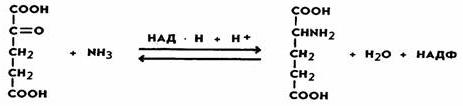
\includegraphics[width=0.7\linewidth]{pictures/glutamin}
\tetrahedral{0==COOH;3==\tetrahedral{0==C;4D==O;1==(yl);3==\tetrahedral{0==$CH_{2}$;1==(yl);3==\tetrahedral{0==$CH_{2}$;1==(yl);3==\tetrahedral{0==COOH;1==(yl)}}}}}  $+ NH_{3} \xrightarrow{\text{НАДН} + H^{+}}$ \tetrahedral{0==COOH;3==\tetrahedral{0==CHNH$_{2}$;1==(yl);3==\tetrahedral{0==$CH_{2}$;1==(yl);3==\tetrahedral{0==$CH_{2}$;1==(yl);3==\tetrahedral{0==COOH;1==(yl)}}}}} + $H_{2}O$ + НАДФ 
\end{minipage}

\caption{Схема образования глутаминовой кислоты}
\label{glutamin}
\end{figure}


%%%%%%%%%%%%%%%%%%%%%%%%%%%%%%%%%%%%%%%%%%%%%%%%%%%%%%%%%%%%%%%%%%%%%%%%%%%%%%%%%%%%%%%%%% 


\paragraph*{}Реакция присоединения аминогруппы $\alpha$-кетоглютаровой кислоте катализируется ферментом глутаматдегидрогеназой. Фермент глутаматдегидрогеназа катализирует восстановительное аминирование $\alpha$-кетоглутаровой кислоты с образованием глютаминовой кислоты. Для этой реакции необходима \gls{atp}:

%На первом этапе реакции субстраты соединяются с образованием иминокислоты, которая затем восстанавливается в глютаминовую кислоту при участии НАД(Ф)Н. Оба этапа обратимы:
 
\note{Глютаматдегидрогеназа (мол. масса 200-300 к\gls{dalton}) обнаружена в листьях и корнях у всех высших растений. Фермент локализован в митохондриях, хотя имеется в цитоплазме и в хлоропластах. Он состоит из 4-6 субъединиц. Это фермент обратимого действия и зависит от рН. Оптимум рН для аминирования на 1,5 единицы выше, чем для дезаминирования}

\paragraph*{}Образование амидов катализируется ферментом глютаминсинтетазой.
Кофакторами глютаминсинтетазы выступают ионы марганца, кобальта, кальция. Фермент обнаружен во всех органах растений и локализован в цитоплазме. 

\note{Кроме $\alpha$-кетоглутаровой кислоты, играющей основную роль в первичном связывании аммиака, в растениях аммиак может присоединятся в виде аминогруппы и к другим карбоновым кислотам, которые с помощью соответствующих ферментов взаимодействуют с $NH_{3}$, образуя так называемые первичные аминокислоты. Они же могут участвовать в различных реакциях переаминирования, когда аминогруппа переносится на них от каких либо аминокислот. К числу этих органических кислот относятся щавелевоуксусная, пировиноградная, гидроксипировиноградная, глиоксиловая и другие, в процессе восстановительного аминирования которых получаются соответственно аспарагиновая кислота, аланин, серин, глицин}

%Принято считать, что образование аспарагина преобладает в том случае, когда происходит распад белков в семенах. В клетках корня и листьев растущего растения идет, главным образом, образование глютамина. Таким образом, образование аспарагина - это путь обезвреживания аммиака, появляющегося при распаде белка - так называемая регрессивная ветвь азотного обмена, тогда как синтез глютамина - это путь обезвреживания аммиака при синтезе белка - прогрессивная ветвь азотного обмена.

\paragraph*{Роль амидов в растении}

\begin{enumerate}
	\item Растения утилизируют аммиак в форме амидов
	\item Азотные соединения транспортируются по растению в виде амидов
	\item Амиды и их предшественники аминокислоты являются материалом для создания многих других аминокислот в реакциях переаминирования, когда аминогруппа аминокислоты обменивается с кетогруппой кетокислоты с образованием аминокислоты
\end{enumerate}

\subsection*{Физиологическая роль микроэлементов}

\subsubsection*{Железо}

%Среднее содержание железа в растениях составляет 20-80 мг на 1 кг сухой массы. 
\paragraph*{Пути поступления железа в организм растения} Ионы $Fe^{3+}$ почвенного раствора восстанавливаются редокс-системами плазмалеммы клеток ризодермы до $Fe^{2+}$ и в такой форме поступают в корень. 

\paragraph*{Роль железа в растении}

\begin{enumerate}
\item Необходимо для функционирования основных редокс-систем фотосинтеза и дыхания;
\item Участвует в синтезе \hyperlink{sect_hlorophilus}{хлорофилла};
\item Для восстановления нитратов и фиксации молекулярного азота клубеньковыми бактериями, входя в состав нитратредуктазы и \hyperlink{nitrogenaza}{нитрогеназы};
\end{enumerate}

\paragraph*{}Недостаточное поступление железа в растения в условиях переувлажнения и на карбонатных почвах приводит к снижению интенсивности \hyperlink{sect_breazing}{дыхания} и \hyperlink{photosyntesis}{фотосинтеза} и выражается в пожелтении (хлорозе) листьев и быстром их опадении.

\subsubsection*{Марганец}

\paragraph*{Пути поступления марганца}

\paragraph*{}Марганец поступает в клетки в форме ионов $Mn^{2+}$ и накапливается в листьях 
%Среднее его содержание составляет 1 мг на 1 кг сухой массы. Марганец накапливается в листьях. 

\paragraph*{Роль марганца в \gls{metabolism}е растения}

\begin{enumerate}
	\item Необходим для \hyperlink{photolisys}{фотолиза воды} с выделением кислорода и восстановления углекислого газа при \hyperlink{photosyntesis}{фотосинтезе};
	\item Способствует увеличению содержания сахаров и их оттоку из листьев;
	\item активирует некоторые ферменты \note{Например, два фермента \hyperlink{krebs_cycle}{цикла Кребса} -- малат- и изоцитратдегидрогеназы - активируются ионами марганца};
	\item Необходим для функционирования нитратредуктазы при восстановлении нитратов;
	\item Является кофактором РНКполимеразы и ауксиноксидазы, разрушающей фитогормон \hyperlink{auxsin}{3-индолилуксусную кислоту};
\end{enumerate}

\paragraph*{}Cимптом марганцевого голодания -- точечный хлороз листьев, когда между жилками появляются желтые пятна, а затем клетки в этих участках отмирают. 

\subsubsection*{Молибден} 

\paragraph*{Пути поступления молибдена в растение}

%Наибольшее содержание молибдена характерно для бобовых (0,5-20 мг на 1 кг сухой массы), злаки содержат от 0,2 до 2 мг на кг сухой массы. 
\paragraph*{}Молибден поступает в растения в форме аниона $MoO_{2}^{-4}$ и концентрируется в молодых, растущих органах. В листе сосредоточен, в основном, в \hyperlink{cell_plastids}{хлоропластах}.

\paragraph*{Роль молибдена в метаболизме растения}

\begin{enumerate}
	\item Входит в состав нитратредуктазы и нитрогеназы, а также необходим для биосинтеза \hyperlink{leggemoglobin}{легоглобина};
	\item Является активатором ферментов аминирования и переаминирования, ксантиноксидаза и различных фосфатаз;
\end{enumerate}

\paragraph*{Симптомы при недостатки молибдена}

\begin{enumerate}
	\item В тканях накапливается большое количество нитратов;
	\item Не развиваются клубеньки на корнях бобовых;
	\item Наблюдаются деформации листовых пластинок. молодые листья по краям приобретают серую, а затем коричневую окраску затем ткани листа отмирают и остаются только жилки в виде хлыстиков.
\end{enumerate}

\subsubsection*{Кобальт} 

\paragraph*{Роль кобальта в метаболизме растения}
%Среднее содержание кобальта в растениях 0,02 мг на 1 кг сухой массы. 
\paragraph*{}В растениях кобальт встречается в форме иона и в  составе витамина В12.
\begin{enumerate}
\item Необходим бобовым растениям для обеспечения размножения \hyperlink{nitrificators}{клубеньковых бактерий};
\item Участвует в синтезе метионина;
\item Наряду с магнием и марганцем активирует фермент гликолиза фосфоглюкомутазу и фермент аргиназу, гидролизующий аргинин;
\end{enumerate}

\paragraph*{}Внешние признаки недостатка кобальта сходны с признаками \hyperlink{nitroHungry}{азотного голодания}.

\subsubsection*{Медь}

\paragraph*{Поступление меди в растение}

\paragraph*{}Медь поступает в клетки в форме иона $Cu^{2+}$. 
%Среднее содержание меди в растениях 0,2 мг на кг сухой массы. 

\paragraph*{}Около 70 \% всей меди, находящейся в листьях, сосредоточены в \hyperlink{cell_plastids}{хлоропластах}.

\remember{Медь входит в состав многих важных окислительно-восстановительных ферментов}

\paragraph*{Роль меди в \gls{metabolism}е}

\begin{enumerate}
\item Входит в состав \gls{plastocyanin}а -- белка-переносчика электронов между фотосистемами \gls{fs2} и \gls{fs1};
\item Входит в состав \hyperlink{enzimes}{ферментов}, катализирующих окисление аскорбиновой кислоты, дифенолов и гидроксилирование монофенолов;
\item Входит в состав ферментов дыхательной цепи \hyperlink{mitohondria}{митохондрий};
\item Входит в состав \hyperlink{nitritreductaza}{нитратредуктазного} комплекса и влияет на синтез \gls{leggemoglobin}а
\item Повышает устойчивость растений к полеганию так как влияет на активность ингибиторов роста фенольной природы;
\item Повышает засухо-, морозо- и жароустойчивость;
\end{enumerate}

\paragraph*{Недостаток меди вызывает} 

\begin{enumerate}
	\item Задержку роста и цветения;
	\item Хлороз;
	\item Потерю тургора и завядание растений;
	\item У злаков при недостатке меди не развивается колос;
	\item у плодовых появляется суховершинность;
	\item При дефиците меди белеют и отмирают кончики листьев, листья и плоды плодовых деревьев покрываются бурыми пятнами;
\end{enumerate}

\subsubsection*{Цинк}

%\paragraph*{}Содержание цинка в надземных частях бобовых и злаковых растений составляет 15-60 мг на кг сухой массы. Повышенная концентрация отмечается в листьях, репродуктивных органах и конусах нарастания, наибольшая - в семенах.

\paragraph*{Поступление цинка в растение}Цинк поступает в растение в форме катиона $Zn^{2+}$. 

\paragraph*{Роль цинка в метаболизме растения}

\begin{enumerate}
\item Необходим для функционирования ряда ферментов \hyperlink{glycolysis}{гликолиза} -- \note{Например гексокиназы, енолазы, триозофосфатдегидрогеназы, альдолазы}
\item Активирует ферменты, катализирующие расщепление угольной кислоты до углекислого газа и воды;
\note{Это помогает использованию углекислого газа в процессе \hyperlink{photosyntesis}{фотосинтеза}}
\item Участвует в образовании аминокислоты триптофана;
\note{Именно с этим связано влияние цинка на синтез белков, а также фитогормона \hyperlink{auxsin}{\gls{inodolAcid}}, предшественником которой является триптофан. Подкормка цинком способствует увеличению содержания ауксинов в тканях и активирует их рост}
\end{enumerate}

\paragraph*{Симптомы дефицита цинка}

\begin{enumerate}
\item Нарушается фосфорный обмен: \hyperlink{phosphoros}{фосфор} накапливается в корнях, задерживается его транспорт в надземные органы, замедляется превращение фосфора в органические формы.
\item Уменьшается содержание сахарозы и \hyperlink{krahmal}{крахмала};
\item Увеличивается количество органических кислот и небелковых соединений азота -- амидов и аминокислот.
\item В 2-3 раза подавляется скорость деления клеток. Это приводит к морфологическим изменениям листьев, нарушению растяжения клеток и дифференциации тканей.
\item Наиболее характерный признак цинкового голодания -- это задержка роста междоузлий и листьев, появление хлороза и развитие розеточности.
\end{enumerate}


\subsubsection*{Бор}

%\paragraph*{}Его среднее содержание составляет 0,1 мг на кг сухой массы. В боре наиболее нуждаются двудольные растения. Много бора в цветках. 
\paragraph*{}В клетках большая часть бора сосредоточена в клеточных стенках. 

\paragraph*{Роль бора в метаболизме растения}

\begin{enumerate}
\item Усиливает рост пыльцевых трубок, прорастание пыльцы, увеличивает количество цветков и плодов;
\item Снижает активность некоторых дыхательных ферментов, оказывает влияние на углеводный, белковый и нуклеиновый обмен;
\end{enumerate}

\paragraph*{Симптомы недостаток бора}

\begin{enumerate}
\item Нарушается формирование репродуктивных органов, оплодотворение, плодоношение и созревание семян;
\item Нарушаются синтез, превращения и транспорт \hyperlink{sect_glycosids}{углеводов;}
\item Так как бор не может реутилизироваться и поэтому при борном голодании прежде всего отмирают конусы нарастания, останавливается рост побегов и корней, листовые пластинки утолщаются, скручиваются, становятся ломкими, цветки не образуются. 
\end{enumerate}

\paragraph*{}Влиянию различных микроэлементов на рост растения будет посвящена одна из приведенных в данном пособии \hyperlink{mineral_elements_influence}{лабораторных работ}.

\subsection*{Вопросы и задания для самоконтроля}

\begin{enumerate}
\item Из курса экологии вы должны уже быть знакомы с таким понятием как <<\hypertarget{}{Бочка Либиха}>>. Используя учебник экологии, например за авторством Н.А. Березиной \cite{berezina_2009} и материал этого раздела, объясните, почему нехватка хотя бы одного из химических элементов является лимитирующим фактором для растения?
\item С помощью учебника ботаники повторите строение корня. Что такое \hypertarget{question_rizoderma}{ризодерма}? Как она образуется?
\item Как вы думаете, о преобладании какого типа \hypertarget{what_is_transport_type}{транспорта} веществ это свидетельствует -- активного или пассивного? Почему?
\item Какие особенности структуры молекулы какого либо вещества делают ее \hypertarget{polarMolecula}{полярной}?
\item Кукую физиологическую роль в метаболизме растений играют сера, азот, калий, кальций, магний?
\item Атомы каких элементов играют важную роль в поддержании третичной структуры белка за счет образования ковалентных связей между различными участками полипептидной цепи?
\item Какова роль леггемоглобина в процессе усвоения растениями азота?
\item Какие важные для метаболизма растения вещества синтезируются в бактероидах?
\item Вспомните, атомы каких металлов входят в состав активных центров ферментов дыхательной цепи?
\end{enumerate}

